\chapter{Das EVM8168-Entwicklungsboard}
\label{ch:board}
\rm

F�r die in den folgenden Kapiteln beschriebenen Arbeitsschritte zur Optimierung und Analyse des Programmes wurde ein EVM8168-Entwicklungsboard verwendet, welches von der Firma Texas Instruments in Zusammenarbeit mit der Firma Spectrum Digital entwickelt wurde.
Dieses Board kann mit Hilfe eines DM816x (DaVinci\texttrademark) ARM-Prozessors entweder selber Programme ausf�hren oder es k�nnen auch die beiden ARM-Prozessoren C6A816x (Integra\texttrademark) oder AM389x (Sitara\texttrademark) emuliert werden. 


\section{Aufbau des EVM8168} \label{sec:evm816}
Wie in \cite{spec} beschrieben bietet das EVM8168-Entwicklungsboard eine Standalone-Plattform um Programme f�r DaVinci\texttrademark, Integra\texttrademark~oder Sitara\texttrademark~Prozessoren der Firma Texas Instruments zu entwickeln und zu debuggen. Hierf�r sind neben dem DaVinci\texttrademark~noch weitere On-Board Perepherie auf dem Board aufgebracht, die im folgenden teilweise n�her erkl�rt werden sollen.
Das EVM8168-Board hat unteranderem folgende Komponenten integiert:

\begin{itemize}
	\item DM8168- (DaVinci\texttrademark-)ARMprozessor (\textbf{Kapitel~\ref{sec:davinci}}) mit NEON-Einheit (\textbf{Kapitel~\ref{subsec:neon}})
	\item C674x-DSP (\textbf{Kapitel \ref{subsec:dsp}})
	\item Gigabit Ethernet
	\item HDMI
	\item VGA
	\item USB
\end{itemize}

F�r die in dieser Arbeit beschriebene Soundklassifikation wichtig sind au�erdem die Anschl�sse f�r  Line-In, Mic-In und Line-Out, sowie der integrierte AIC3106 Codec, welcher den eingehenden Soundstream f�r den DSP vorbereitet.
\textbf{Abbildung~\ref{fig:top_ti816x_evm}} zeigt eine Draufsicht auf das Entwicklungsboard und die unterhalb dessen angebrachte Daughtercard mit weiteren Anschlussm�glichkeiten.

\begin{figure}[htbp]
	\centering
		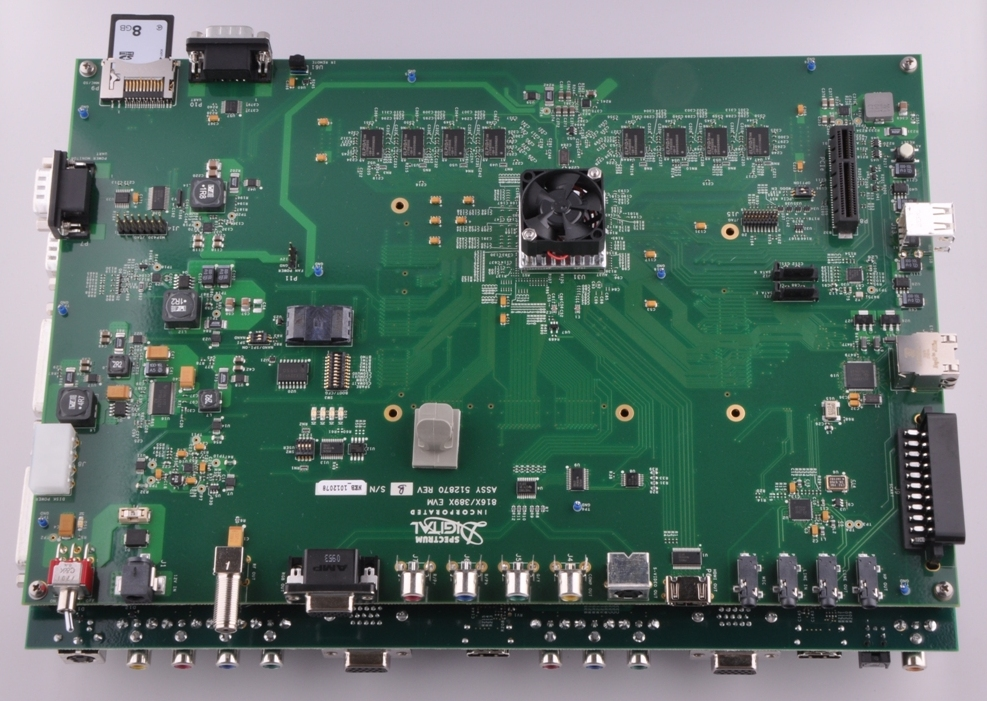
\includegraphics[scale=0.4]{../Pictures/top_ti816x_evm.png}
	\caption{Draufsicht auf das EVM8168}
	\label{fig:top_ti816x_evm}
\end{figure}



\section{Der DaVinci\texttrademark}\label{sec:davinci}
\subsection{Die NEON-Einheit}\label{subsec:neon}
\subsection{Der C674x-DSP-Prozessor}\label{subsec:dsp}